%!TEX root = ../thesis.tex
%*******************************************************************************
%****************************** Third Chapter **********************************
%*******************************************************************************
\chapter{Phase Transition}

% **************************** Define Graphics Path **************************
\ifpdf
    \graphicspath{{Chapter3/Figs/thermodynamics/}{Chapter3/Figs/}}
\else
    \graphicspath{{Chapter3/Figs/thermodynamics/}{Chapter3/Figs/}}
\fi

\textbf{What is this}
Phase transition is one of the most studied problem in physics. Phase transition is a process where below a critical point the system behaves in one way whereas above that point the system behaves in a completely different way. There is a control parameter in phase transition. It can be temperature $T$ or magnetic field $H$. For example in ferromagnet to paramagnet transition temperature is the control parameter and for normal to superconductor transition both temperature and magnetic field are the control parameter.\\
The first explicit statement of the first law of thermodynamics, by \textit{Rudolf Clausius} in 1850, referred to cyclic thermodynamic processes. \\
\textit{In all cases in which work is produced by the agency of heat, a quantity of heat is consumed which is proportional to the work done; and conversely, by the expenditure of an equal quantity of work an equal quantity of heat is produced.}\\
\begin{align}
	\Delta E = Q + W
\end{align}
where, $Q$ is the net quantity of heat supplied to the system by its surroundings and $W$ is the net work done by the system.
The IUPAC convention for the sign is as follows: All net energy transferred to the system is positive and net energy transferred from the system is negative.
Clausius also stated the law in another form, referring to the existence of a function of state of the system, the internal energy, and expressed it in terms of a differential equation for the increments of a thermodynamic process.\\
\textit{In a thermodynamic process involving a closed system, the increment in the internal energy is equal to the difference between the heat accumulated by the system and the work done by it.}\\
For quasi-static process
\begin{align}
	dE = dQ - P dV
\end{align}
$E$ is the internal energy.
here $W = -P dV$
since work done by the system on the environment if the product $P dV$ whereas the work done on the system is $-P dV$ for pressure $P$ and volume change $dV$.\\
The term heat for $Q$ means "that  amount of energy added or removed by conduction of heat or by thermal radiation", rather than referring to a form of energy within the system. 
The internal energy is a mathematical abstraction that keeps account of the exchanges of energy that befall the system.

For quasi-static state we can write
\begin{equation}
dQ = T dS
\ref{eqn:def_enthalpy}
\end{equation}
where $S$ is the entropy of the system and $T$ is the temperature.
Thus we can write for canonical ensemble
\begin{equation}
dE = TdS - pdV
\end{equation}
such that $E=E(S,V)$  and 
for grand canonical ensemble 
\begin{equation}
dE = TdS - pdV + \mu dN
\end{equation}
where $E=E(S,V,N)$.
But a problem arises, since there is no device we currently posses that can measure entropy. So we use Legendre transformation to change variable dependency
\begin{align}
	dE  	&= TdS - pdV  \nonumber \\ 
	&= TdS + SdT - SdT - PdV  \nonumber \\ 
	d(E-TS) &= -SdT - PdV  \nonumber \\
	dA 		&= -SdT - PdV \label{eqn:helmholtz_def}
\end{align}
where $A=A(T,V)$  is the Helmholtz free energy. We can perform another Legendre transformation in \ref{eqn:helmholtz_def} as follows
\begin{align}
	dA 		&= -SdT - PdV -VdP + VdP \nonumber \\
	d(A+PV) &= -SdT + VdP \nonumber \\
	dG      &= -SdT + VdP \label{eqn:gibbs_def}
\end{align}
where $G=G(T,P)$ is the Gibbs free energy.\\
Let's take a break to talk about free energy. What is free energy?
\section{Classification}
	\subsection{First Order}
		\begin{enumerate}
			\item Latent heat of nucleation in growth
			\item Symmetry may or may not be broken
			\item Discontinuous change in entropy
		\end{enumerate}
	\subsection{Second Order}
		\begin{enumerate}
			\item Sysmmetry is always broken
			\item No Latent heat or meta-stable state
			\item Continuous change in entropy
		\end{enumerate}
	
\section{Definition of Thermodynamic Quantities}
	\subsection{Entropy}
	Entropy is considered as a quantity about the disorderness of a system. This kind of disorder is the number of states a system can take on. So what are the states of a system? Imagine a cube of volume $1cm^3$, filled with one particular gas. At a particular time if we can label all the molecules of the gas uniquely then at next moment most of the molecule will change their positions due to their random motion. Then we will not be able to identify each molecule with their previous label. This process of identifying the labels of the molecules are easier if it's a liquid and even more easier in it's solid form. Since temperature increases the random motion of the molecules, as the temprature rises it is more difficult to identify those molecules. Thus at high temperature a system has higher entropy. Another thing to mention about it's volume. If a larger volume is selected then obviously the number of possible states will increase therefore entropy will increase.\\
	Example:\\
	If we were ot compare the entropy of the moon and the sun, the above discussion tells us that the sun has higher entropy than the moon. The reason is that the sun is much much larger than the moon and has much higher temperature than the moon. Therefor the number of possible states will be larger for the sun than the moon.\\
	Entropy in one of the key feature of a phase transition model. But thermodynamic entropy cannot be calculated for any model such as our percolation on a square lattice model. So we take our approach in another way. Information entropy or the Shanon entropy is best suited for our model. The concept of information entropy was introduced by Claude Shannon in his 1948 paper "A Mathematical Theory of Communication" \cite{shanon_entropy}. The Defition is
	\begin{align}
		H = - \sum_{i} \mu_i \log \mu_i	
	\end{align}
	where, $\mu_i$ is the probability of getting $i$-th element.\\
	Say we have a coin with a head and a tail. If the coin is unbiased then the probability of getting the head or the tail is 50\% or 0.5. Now what's the entropy of this system? The Shanon entropy is the one that can be used here. For convenience $\log_{2}$ will be used for evaluating logarithms here, after all $\log_{2} = const. \log_{10} = const. \log_{e}$. Here, $\mu_i = 0.5$ and $\log_{2} (0.5) = -1$, Therefore we have
	\begin{align}
		H &= - (0.5 \log_{2} (0.5) + 0.5 \log_{2} (0.5)) \nonumber \\ 
		&= - (0.5 \times (-1) + 0.5 \times (-1)) \nonumber \\ 
		&= 1 \nonumber
	\end{align}
	so in this system entropy is $1$.\\
	Now take a new system where there is $4$ identical object. Since all objects are identical, each have probability $\mu_i = 1/4$ and $\log_{2} (1/4) = -2$. Then the total entropy of that system is $2$. So this is clear that the entropy increses with the increase of the system size. Here system size is determined by the number of particles in it. Now, let's take a non-uniform system, where there are total $8$ particles and there are $4$ cluster. Cluster $1$ has $4$ particles and cluster $2$ has $2$ particles and other $2$ cluster of $1$ particle each. Probability of getting cluster $1$ is $\mu_1 = 4/8$ and for cluster $2$ it is $\mu_2 = 2/8$ and for other clusters it is $\mu_3 = \mu_4 = 1/8$. Now the entropy of the system becomes,
	\begin{align}
		H &= - \sum_i \mu_i \log_2 \mu_i \nonumber \\
		&= - (4/8 \log_2 (4/8) + 2/8 \log_2 (2/8) + 1/8 \log_2(1/8) + 1/8 \log_2(1/8) \nonumber \\
		&= - (-1/2 -1/2 -3/8 -3/8) \nonumber \\
		&= 7/4 \nonumber
	\end{align}
	which is less then the entropy of a system where all $8$ particles are disconnected, i.e., $H=3$. So we can see that as the particles are joined together entropy reduces, which is in agreement with the experimental results. 
	\begin{figure}
		\begin{subfigure}{.5\textwidth}
			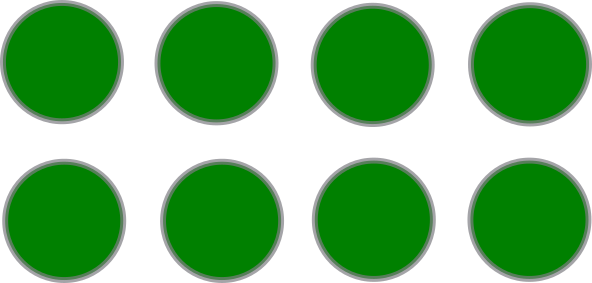
\includegraphics[width=.5\linewidth]{entropy_cluster/step1.png}
			\caption{Free particles. $H=3$}
		\end{subfigure}
		\begin{subfigure}{.5\textwidth}
			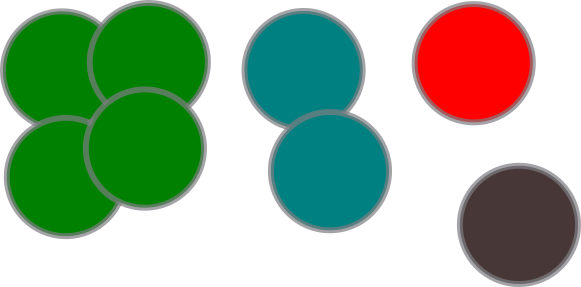
\includegraphics[width=.5\linewidth]{entropy_cluster/step2.png}
			\caption{Some Free and Some Bound Particles. $0 < H < 3$}
		\end{subfigure}
		\begin{subfigure}{.5\textwidth}
			
\includegraphics[width=.5\linewidth]{entropy_cluster/step3.png}
			\caption{Bount particles. $H=0$}
		\end{subfigure}
		\caption{entropy of a system of $8$ particles}
	\end{figure}
	
	The reason I am taking the system size as $2^n$ for all $n$ is that it's easier to take logarithm of base $2$.
	
	
	\subsection{latent heat}
	The latent heat associated with the phase transition is , where and are the entropies just above and below the phase transition. Since the entropy is continuous at the phase transition, the latent heat is zero. The latent heat is always zero for a second order phase transition.
	\subsection{Specific Heat}
	\subsection{Order Parameter}
	\subsection{Susceptibility}
	The first law of thermodynamics for a non magnetic system is \ref{label}
	\begin{equation}
		dE = TdS - PdV
	\end{equation}
	for a magnetic system $P \rightarrow h$ and $V \rightarrow -m$, where $h$ is the magnetic field and $m$ is the magnetization. The negative sign for the magnetization is because of the fact that the magnetization increases with the increase of the magnetic field whereas the volume decreases as the pressure increases. Since we relate pressure to the magnetic field, to relate volume to magnetization we need to put a minus sign with it. Thus we get
	\begin{align}
		dE &= TdS + hdm \\
		   &= TdS + SdT - SdT + h dm \\
		d(E - TS)  &= -SdT + h dm \\
		dA &= -SdT + h dm \label{eqn:helmholtz_mag_system} \\
		dA &= -SdT + h dm + m dh -m dh \\
		d(A - mh) &= -SdT - m dh\\
		dG &= -SdT -m dh \label{eqn:gibbs_mag_system}
	\end{align} 
	where $A=A(T,m)$ is the  Helmholtz free energy and $G=G(T,h)$ is the Gibbs free energy for the magnetic system. From the definition of free energy for a magnetic system \ref{eqn:gibbs_mag_system} \ref{eqn:helmholtz_mag_system} we can find the expression for entropy and magnetization in terms of free energy.
	\begin{equation}
		S = -\left(\frac{\partial G}{\partial T}\right)_h = -\left(\frac{\partial A}{\partial T}\right)_m
	\end{equation}
	\begin{equation}
		m = -\left(\frac{\partial G}{\partial h}\right)_T
		\label{eqn:magnetization_def}
	\end{equation}
	\begin{equation}
		h = \left(\frac{\partial A}{\partial m}\right)_T
		\label{eqn:mag_field_def}
	\end{equation}	
	And since the susceptibility is defined as the derivative of the magnetization with respect to the magnetic field, we get
	\begin{equation}
		\chi = \left(\frac{\partial m}{\partial h}\right)_h = - \left(\frac{\partial^2G}{\partial h ^2}\right)_T
		\label{eqn:susceptibility_def}
	\end{equation}
	again we can write $\chi$ as
	\begin{align}
		\chi &= \frac{1}{\frac{\partial h}{\partial m}} \nonumber \\
			 &= \frac{1}{\frac{\partial^2 A}{\partial m ^2}} \label{eqn:susceptibility_def2}
	\end{align}
	
	\subsection{1 Dimensional Lattice}
	\subsection{Exact solution in 1 Dimension}
	\subsection{Bethe Lattice}
	\subsection{Exact solution in infinite Dimension}
	
	
	%-------------------------------------------------------------------------------------------
\section{Shapes of the Thermodynamic Quantities}
	\subsection{Calculus to determine the shapes}
	\label{sec:determine_shape_using_calculus}
	From the law of Calculus we can estimate the approximate shape of a function by it's first and second derivative.
	Say we have a function $f(x)$ and we want to estimate it's shape.
	If the first derivative of this function is negative (positive) the function is said to have decreasing (increasing) slope \ref{fig:diff1_of_f}.
	\begin{figure}
		\centering
		\begin{subfigure}{0.329\textwidth}
			\centering
			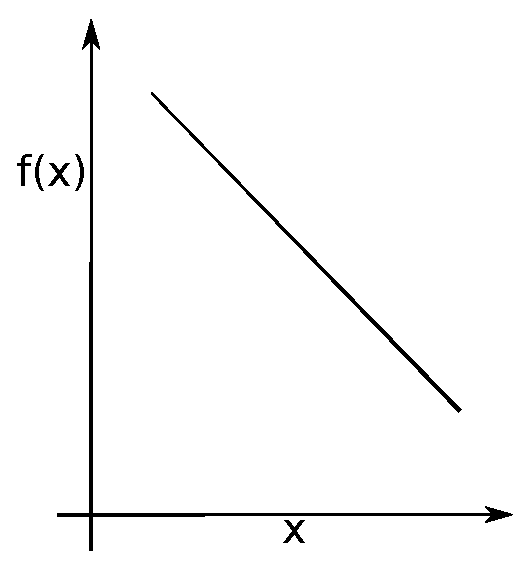
\includegraphics[width=\linewidth]{{{thermodynamics/decreasing}}}
			\caption{negative slope}
		\end{subfigure}
		\begin{subfigure}{0.329\textwidth}
			\centering
			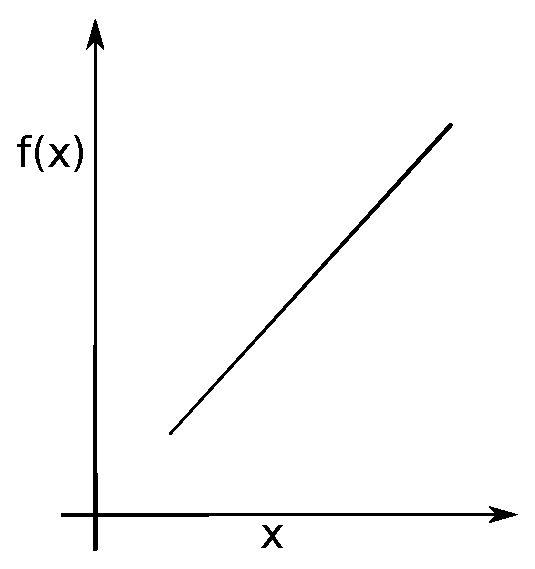
\includegraphics[width=\linewidth]{{{thermodynamics/increasing}}}
			\caption{positive slope}
		\end{subfigure}
		\caption{shape of $f(x)$ from $f^{\prime}(x)$}
		\label{fig:diff1_of_f}
	\end{figure}
	
	If the second derivative of this function is negative (positive) the function is said to have concave (convex) shape \ref{fig:diff2_of_f}.
	\begin{figure}
		\centering
		\begin{subfigure}{0.329\textwidth}
			\centering
			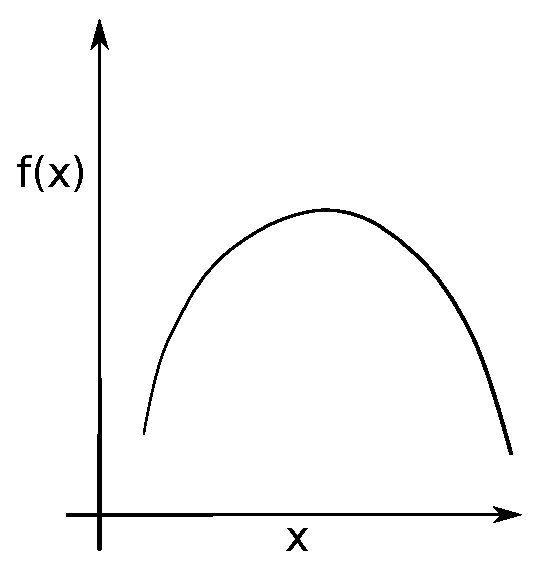
\includegraphics[width=\linewidth]{{{thermodynamics/concave}}}
			\caption{concave}
		\end{subfigure}
		\begin{subfigure}{0.329\textwidth}
			\centering
			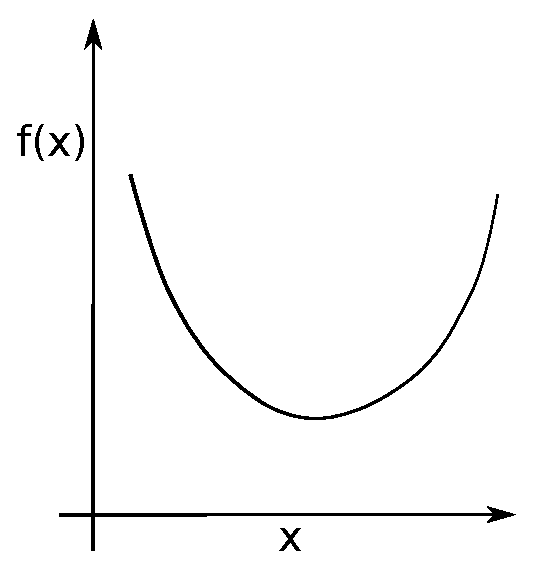
\includegraphics[width=\linewidth]{{{thermodynamics/convex}}}
			\caption{convex}
		\end{subfigure}
		\caption{shape of $f(x)$ from $f^{\prime\prime}(x)$}
		\label{fig:diff2_of_f}
	\end{figure}
	Thus if we know the sign of the first and second derivative we can approximate a shape of the function.
	\subsection{Free Energy}
	Now since we obtain from \ref{eqn:gibbs_def} that the entropy is the first derivative of the free energy \ref{eqn:entropy_by_gibbs} and from \ref{eqn:def2_specific_heat} specific heat is the second derivative of the free energy \ref{eqn:specific_heat_by_gibbs}. Now since the entropy is a positive quantity and specific heat is also a positive quantity we get that the first and second derivative of the free energy is negative which implies from the laws of calculus that the shape of the free energy should be a decreasing concave curve \ref{fig:free_energy} in other words concave shaped with negative slope.
	\begin{equation}
	S = - \frac{\partial G}{\partial T}
	\label{eqn:entropy_by_gibbs}
	\end{equation}
	\begin{equation}
	C = - \frac{\partial^2 G}{\partial T ^2}
	\label{eqn:specific_heat_by_gibbs}
	\end{equation}
	\begin{figure}
		\centering
		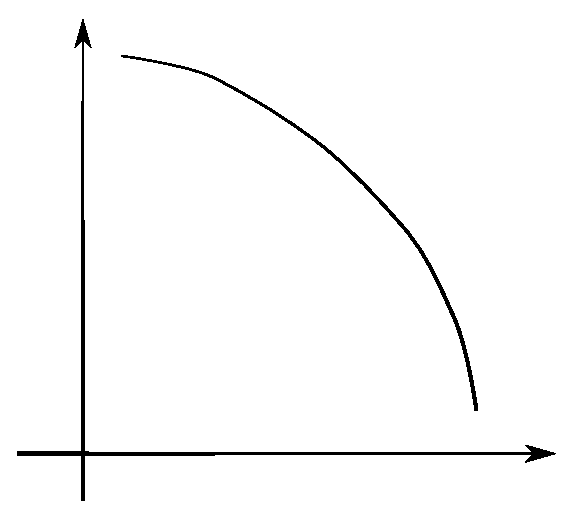
\includegraphics[width=0.3\columnwidth]{{{thermodynamics/free_energy}}}
		\caption{Shape of the free energy}
		\label{fig:free_energy}
	\end{figure}

	\subsection{Entropy and Specific Heat}	
	Now that we know the shapes of the free energy, the very next thing to do is to find the shape of the entropy. Since we can get entropy from differentiating the free energy with respect to temperature $T$ we get the following shape \ref{fig:entropy_1_2}. From the definition of the transition order we know that the first order transition is discontinuous and the second order transition continuous. Since the first order transition requires latent heat at the critical point the discontinuity is inevitable. Note that, since entropy measures disorderedness of a system it should increase with increasing temperature. Because the temperature is nothing but the average kinetic energy of the particles in the system. As the kinetic energy of the system increases with temperature, the particles tend to vibrate more and get higher average velocity. Thus making the system disordered. Therefore in a physical system entropy always increases with the increasing of temperature. If we find something different, as if, the entropy is decreasing with the increasing of temperature, there must be a problem somewhere.
	\begin{figure}
		\centering
		\begin{subfigure}{0.329\textwidth}
			\centering
			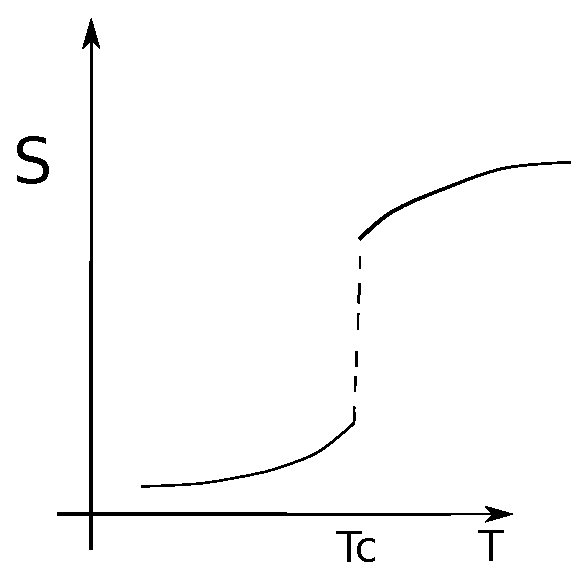
\includegraphics[width=\linewidth]{{{thermodynamics/entropy_1st}}}
			\caption{Entropy in first order transition}
		\end{subfigure}
		\begin{subfigure}{0.329\textwidth}
			\centering
			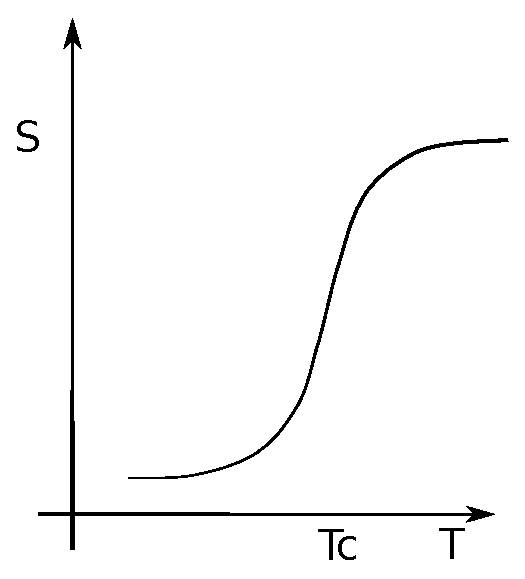
\includegraphics[width=\linewidth]{{{thermodynamics/entropy_2nd}}}
			\caption{Entropy in 2nd order transition}
		\end{subfigure}
		\caption{Shape of entropy}
		\label{fig:entropy_1_2}
	\end{figure}
	Just after knowing the shape of entropy one can anticipate the shape of specific heat, which is the derivative of the entropy with respect to temperature and is defined in \ref{eqn:def2_specific_heat_by_entropy}. Using this and the shape of entropy we can get the shape of the specific heat immediately as follows
	\begin{figure}
		\centering
		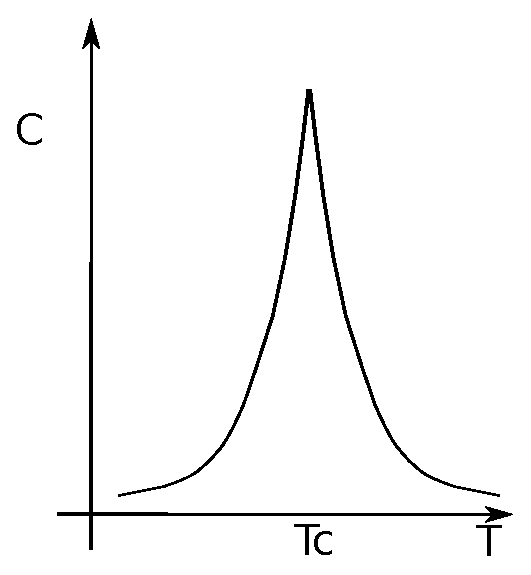
\includegraphics[width=\linewidth]{{{thermodynamics/specific_heat}}}
		\caption{Shape of Specific Heat}
		\label{fig:specific_heat}
	\end{figure}
	\subsection{Order Parameter and Susceptibility}
	Since diamagnetic substances have negative susceptibilities $(\chi < 0)$; paramagnetic, and ferromagnetic substances have positive susceptibilities $(\chi > 0)$, and we are working for a phase transition model similar to paramagnet and ferromagnet transition, taking susceptibility to be positive is appropriate for our model. Now if susceptibility is positive then from \ref{eqn:susceptibility_def} we get $\left(\frac{\partial^2G}{\partial h ^2}\right) < 0$ which means that the shape of the free energy for this case is concave from the knowledge of \ref{sec:determine_shape_using_calculus}. And from \ref{eqn:magnetization_def} and the fact that the magnetic field $h$ can be positive or negative, as it can change direction, the Gibbs free energy is negative, since it is the lowest binding energy. \\
	Also from \ref{eqn:susceptibility_def2} we can say $\frac{\partial^2 A}{\partial m ^2}$ is positive giving convex shape of the Helmholtz free energy. And \ref{eqn:mag_field_def} tells us that since $h$ can ve positive or negative, the Helmholtz free energy can have increasing or decreasing slope respectively.
	\begin{figure}
		\centering
		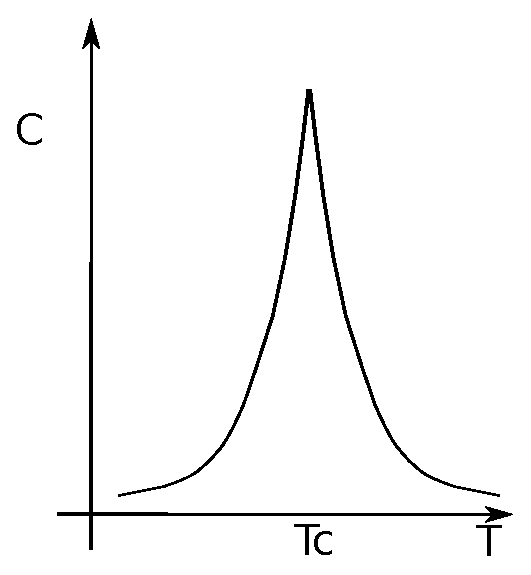
\includegraphics[width=\linewidth]{{{thermodynamics/specific_heat}}}
		\caption{figure required}
	\end{figure}
	


%-----------------------------------------------------------------------------------
\section{Response Functions}
The Specific heat and Susceptibility are called the response function in thermodynamics and the definitions are as follows. The specific heat $C_p$ or $C_v$ is the derivative of the enthalpy with respect to the temperature at constant pressure or volume respectively.
\begin{equation}
C_x = \left(\frac{dQ}{dT}\right)_x
\label{eqn:def_specific_heat}
\end{equation}
here $x$ can be $P$ for pressure or $V$ for volume. And from \ref{eqn:def_enthalpy} we can write
\begin{equation}
C_x = T \left(\frac{dS}{dT}\right)
\label{eqn:def2_specific_heat_by_entropy} 
\end{equation}
To give the following
\begin{align}
C_v = -T\left(\frac{\partial^2 A}{\partial T^2}\right)_v \\
C_p = -T\left(\frac{\partial^2 G}{\partial T^2}\right)_p
\label{eqn:def2_specific_heat} 
\end{align}

Nearest neighbor interation and 2nd nearest neighbor interaction.
Old models of phase transition : Ising model 1D and 2D. Bragg Willium model. 

%------------------------------------------------------------------------------------
\section{Critical Exponents}
	Near the critical point there is, in general, a function that describes the behavior of the system that is mostly interesting. For thermodynamical system the temperature is the control parameter \ref{??}, thus that function depends on the temperature. But since we want the information at the critical point, $(T-T_c)/T_c$, instead of $T$ is a better parameter to address. In equation
	\begin{equation}
		\epsilon = \frac{T-T_c}{T_c} = \frac{T}{T_c} - 1
	\end{equation}
	$\epsilon$ is considered a better parameter. Thus a function $f(\epsilon)$ is used instead of $f(T)$. Using the fact that near $T_c$ the function $f(\epsilon)$ exhibits power law \ref{??}
	\begin{equation}
		f(\epsilon) \sim \epsilon^\lambda
	\end{equation}
	The following figures shows some function that exhibit power law
	\begin{figure}
		\centering
		\begin{subfigure}{0.4\textwidth}
			\centering
			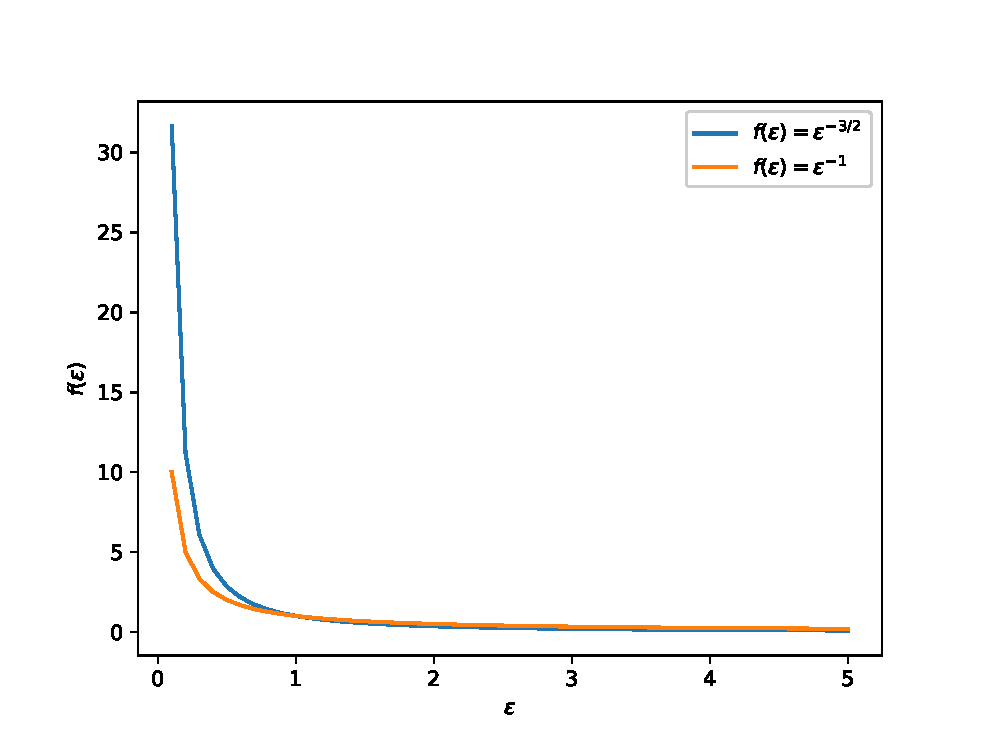
\includegraphics[width=\linewidth]{{{power_law_functions/fig1}}}
			\caption{$f(\epsilon) \sim \epsilon^\lambda$ where $\lambda=-1,-3/2$}
		\end{subfigure}
		\begin{subfigure}{0.4\textwidth}
			\centering
			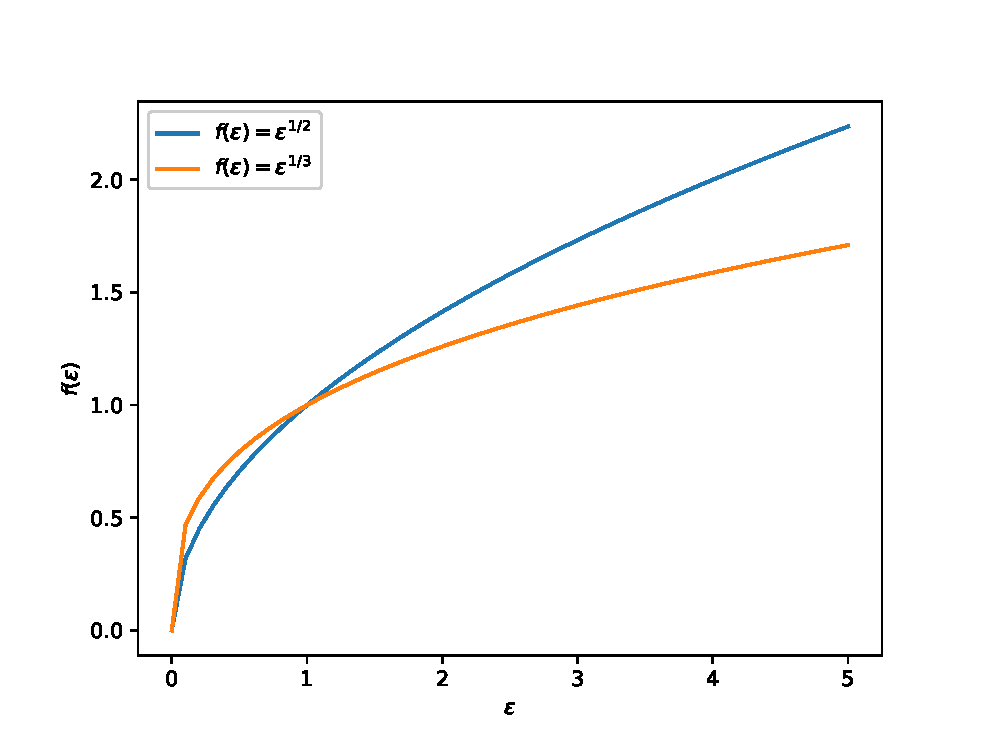
\includegraphics[width=\linewidth]{{{power_law_functions/fig2}}}
			\caption{$f(\epsilon) \sim \epsilon^\lambda$ where $\lambda=1/2,1/3$}
		\end{subfigure}
		\caption{Function showing power law}
	\end{figure}
	To see this more closely, we can expand any function $f(\epsilon)$ as a power series of $\epsilon$
	\begin{equation}
		f(\epsilon) = A \epsilon^\lambda ( 1 + B \epsilon^a + C \epsilon^b + ...)
	\end{equation}
	Near $T_c$ only the first term is dominating \ref{??}.\\
	We had the Gibbs free energy (for a magnetic system)
	\begin{equation}
		G = G(T,h) \equiv G(\epsilon, h)
	\end{equation}
	since $\epsilon$ is a better parameter. Assume that $G$ is a generalized Homogeneous function. Therefore from \ref{??} we can write
	\begin{equation}
		G(\lambda^{a_\epsilon} \epsilon, \lambda^{a_h} h) = \lambda G(\epsilon, h)
		\label{eqn:gibbs_homogenious}
	\end{equation}
	differentiating equation \ref{eqn:gibbs_homogenious} with respect to $h$
	\begin{align}
		\frac{\partial G(\lambda^{a_\epsilon} \epsilon, \lambda^{a_h} h)}{\partial h} &= \lambda \frac{\partial G(\epsilon, h)}{\partial h} \nonumber \\
		\frac{\partial G(\lambda^{a_\epsilon} \epsilon, \lambda^{a_h} h)}{\partial \lambda^{a_h} h} \lambda^{a_h} &= \lambda \frac{\partial G(\epsilon, h)}{\partial h} \nonumber \\
		\lambda^{a_h} G^\prime(\lambda^{a_\epsilon} \epsilon, \lambda^{a_h} h) &= \lambda G^\prime (\epsilon, h) \nonumber \\
		-\lambda^{a_h} m(\lambda^{a_\epsilon} \epsilon, \lambda^{a_h} h) &= -\lambda m(\epsilon, h) \nonumber \\
		m(\lambda^{a_\epsilon} \epsilon, \lambda^{a_h} h) &= \lambda^{1-a_h} m(\epsilon, h) \\
		\label{eqn:order_parameter_homogeneous}
	\end{align}
	Here $m$ is the magnetization or order parameter.\\
	\textbf{Figure of order general parameter}\\
	Setting $h=0$ in equation \ref{eqn:order_parameter_homogeneous}
	\begin{align}
		m(\lambda^{a_\epsilon} \epsilon)	 &= \lambda^{1-a_h} m(\epsilon) \nonumber \\
		m(1)	 &= \lambda^{1-a_h} m(\epsilon) \nonumber \\
		m(1)	 &= \epsilon^{-\frac{1-a_h}{a_\epsilon}} m(\epsilon) \nonumber \\
		m(\epsilon) &= \epsilon^\beta m(1) \label{eqn:order_parameter_and_beta}
	\end{align}
	where
	\begin{equation}
		\beta = \frac{1-a_h}{a_\epsilon}
		\label{eqn:beta}
	\end{equation}
	Note that, setting $\lambda^{a_\epsilon} \epsilon = 1$ gives $\lambda = \epsilon^{-1/a_\epsilon}$.\\
	Setting $\epsilon=0$ in equation \ref{eqn:order_parameter_homogeneous}
	\begin{align}
		m(\lambda^{a_h} h) &= \lambda^{1-a_h} m(h) \nonumber \\
		m(1) &= h^{-\frac{1-a_h}{a_h}} m(h) \nonumber \\
		m(h) &= m(1) h^\delta \label{eqn:order_parameter_and_delta}
	\end{align}
	where
	\begin{equation}
		\delta = \frac{a_h}{1-a_h}
		\label{eqn:delta}
	\end{equation}
	Again, note that, setting $\lambda^{a_h} h = 1$ gives $\lambda = h^{-1/a_h}$\\
	Now, Since the response functions are the second derivative of the free energy \ref{??}, by differentiating \ref{eqn:gibbs_homogenious} twice with respect to $\epsilon$ we get the Specific Heat
	\begin{align}
		\lambda^{2 a_\epsilon} G^{\prime\prime}(\lambda^{a_\epsilon} \epsilon, \lambda^{a_h} h) &= \lambda G^{\prime \prime}(\epsilon, h) \nonumber \\
		\lambda^{2 a_\epsilon} \frac{\partial G(\lambda^{a_\epsilon} \epsilon, \lambda^{a_h} h)}{\left(\frac{1}{T_c}\right)^2 \partial T^2} &= \lambda G^{\prime \prime}(\epsilon, h) \nonumber \\
		\lambda^{2 a_\epsilon} C(\lambda^{a_\epsilon} \epsilon, \lambda^{a_h} h) &= \lambda C(\epsilon, h)
		\label{eqn:specific_heat_homogeneous}
	\end{align}
	We have used $\epsilon = \frac{T}{T_c} -1$ and $d\epsilon = \frac{1}{T_c} dT$. Now setting $h=0$ we get from \ref{eqn:specific_heat_homogeneous}
	\begin{align}
		\lambda^{2 a_\epsilon} C(\lambda^{a_\epsilon} \epsilon) &= \lambda C(\epsilon) \nonumber \\
		C(1) &= \lambda^{1- 2 a_\epsilon} C(\epsilon) \nonumber \\
			 &= \epsilon^{-\frac{1-2 a_\epsilon}{a_\epsilon}} C(\epsilon) \nonumber \\
		C(\epsilon) &= \epsilon^{-\alpha} C(1) \label{eqn:specific_heat_and_alpha}
	\end{align}
	We have used the value of $\lambda$ when we set $\epsilon \lambda^{a_\epsilon}=1$ and the exponent
	\begin{equation}
		\alpha = \frac{2 a_\epsilon - 1}{a_\epsilon}
		\label{eqn:alpha}
	\end{equation}
	
	Again by differentiating \ref{eqn:gibbs_homogenious} twice with respect to $h$ we get the susceptibility. Then we set $h=0$ to get only $\epsilon$ dependency.
	\begin{align}
		\lambda \frac{\partial^2 G(\epsilon,h)}{\partial h^2} &= \lambda^{2 a_h} \frac{\partial^2 G(\lambda^{a_\epsilon} \epsilon, \lambda^{a_h} h)}{\partial h^2} \nonumber \\
		\lambda \chi(\epsilon, h) &= \lambda^{2 a_h} \chi(\lambda^{a_\epsilon}\epsilon, \lambda^{a_h} h) \nonumber \\
		\chi(\epsilon) &= \lambda^{2 a_h - 1} \chi(\lambda ^{a_\epsilon} \epsilon) \nonumber \\
		\chi(\epsilon) &= \epsilon^{-\gamma} \chi(1) 
		\label{eqn:susceptibility_homogeneous}
	\end{align}
	Similar to previous case, We have used the value of $\lambda$ when we set $\epsilon \lambda^{a_\epsilon}=1$ and the exponent is
	\begin{equation}
		\gamma = \frac{2 a_h -1}{a_\epsilon}
		\label{eqn:gamma}
	\end{equation}
	\subsection{List of Thermodynamic Quantities that Follows Power Law}
	\textbf{Critical Exponents at a glance} is it better title.\\
		The exponent that scales Specific heat is called $\alpha$ 
		\begin{equation}
			C \sim \epsilon^{-\alpha}
		\end{equation}
		The exponent that scales order-parameter is called $\beta$ 
		\begin{equation}
			m \sim \epsilon^{\beta}
		\end{equation}
		Another exponent that scales order-parameter is called $\delta$, but it relates the order parameter with the magnetic field, $h$
		\begin{equation}
			m \sim h^{\delta}
		\end{equation}
		The exponent that scales susceptibility is called $\gamma$ 
		\begin{equation}
			\chi \sim \epsilon^{-\gamma}
		\end{equation}
		Note that these quantities only follows power law near $T_c$.
	\subsection{Rushbrooke Inequality}
		\begin{equation}
			\alpha + 2 \beta + \gamma \ge 2
		\end{equation}
		but the equality is often obtain theoretically which is shown below in the present case 
		\begin{align}
			\alpha + 2\beta + \gamma &= \frac{2 a_\epsilon -1}{a_\epsilon} 
					+ \frac{2 (1 - a_h)}{a_\epsilon}
					+ \frac{2 a_h - 1}{a_\epsilon} \nonumber \\
					&= \frac{2 a\epsilon}{a\epsilon} \nonumber \\
					&= 2 \nonumber
		\end{align}
	Thus the Rushbrooke inequality is satisfied.
	\subsection{Griffiths Inequality}
	\begin{equation}
		\alpha + \beta (1+\delta)  = 2
	\end{equation}
	Let's do a quick check to see if this is also satisfied.
	\begin{align}
		\alpha + \beta (1+\delta) &= \frac{2 a_\epsilon - 1}{a_\epsilon} 
									+ \frac{1 - a_h}{a_\epsilon} \left(1 + \frac{a_h}{1 - a_h}\right) \nonumber \\
								  &= \frac{2 a_\epsilon - 1}{a_\epsilon}  + \frac{1}{a_\epsilon} \nonumber \\
								  &= \frac{2 a_\epsilon}{a_\epsilon} \nonumber \\
								  &= 2 \nonumber \\
	\end{align}
	So the Griffiths Inequality is also satisfied. 
\section{Models}
	\subsection{Ising model in 1D lattice}
	\subsection{Ising model in 2D lattice}
	\subsection{Bragg William Model}
